\begin{exercise}{Verengtes Rohr}{10}
  Ein Zylinderförmiges Rohr mit einem Durchmesser von $R_{1}=50$ mm ist auf
  einem Zwischenstück verengt und besitzt dort nur noch einen Radius von
  $R_{2}=25$ mm. An der verengten Stelle ist von unten ein weiteres Rohr mit
  einem Radius von $R_{3}=10$ mm angeschlossen, dessen Ende sich in einem
  Wasserbecken befindet. Durch das Rohr flie\ss en 6 L Wasser pro Sekunde.

  \begin{enumerate}
    \item [a)] Welcher Unterdruck entsteht an der verengten Stelle?
    \item [b)] Kann durch das senkrechte Rohr das untere Wasser 1 m hoch gezogen
    werden?
  \end{enumerate}
\end{exercise}

\FloatBarrier

  \begin{figure}[h]
    \centering
    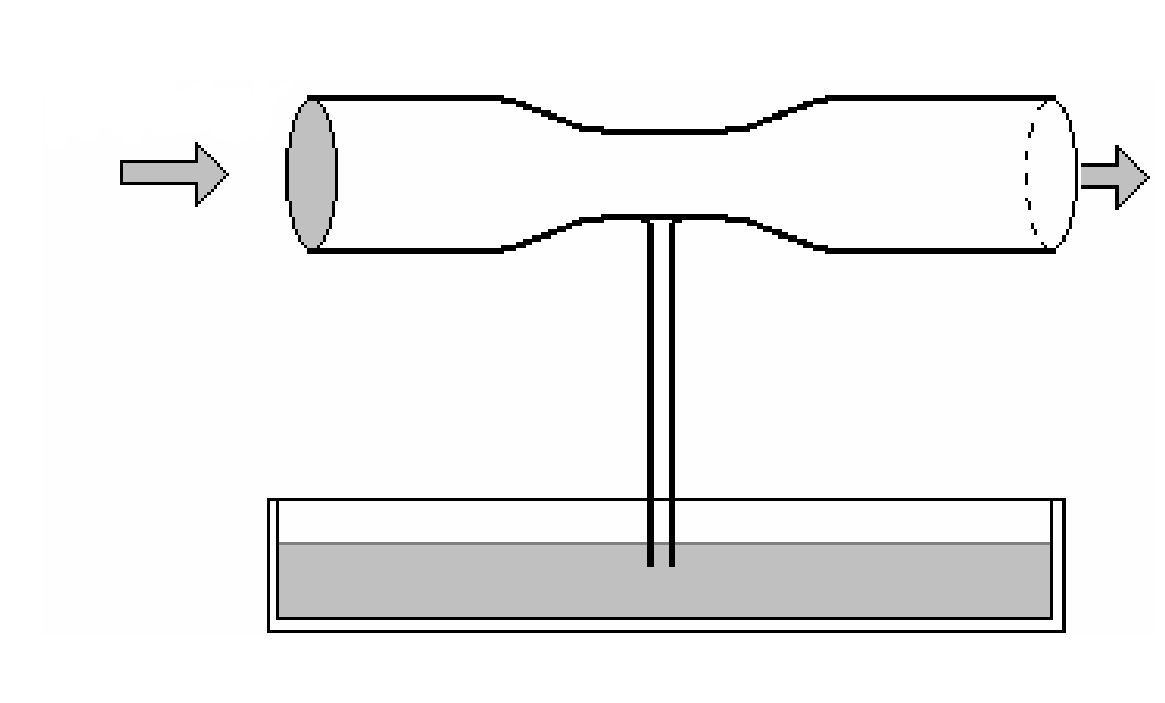
\includegraphics[width = 0.5\textwidth]{Rohr.jpg}
  \end{figure}


\begin{exercise}{Zusatzaufgabe}{+10}
  \begin{enumerate}
    \item [a)] Bestimmen Sie das elektrische Feld eines unendlich langen Drahtes.
    \item [b)] Bestimmen Sie das magnetische Feld eines unendlich langen Drahtes
               mit dem Durchmesser $R_{0}$. Betrachten Sie dabei auch das Feld
               innerhalb des Leiters.
    \item [c)] Bestimmen Sie das magnetische Feld einer Torroidspule mit innerem
               Radius $r_{1}$ und äu\ss erem Radius $r_{2}$. Betrachten Sie dabei
               alle Bereiche (r<$r_{1}$,$r_{1}$<r<$r_{2}$,r>$r_{2}$).
  \end{enumerate}
\end{exercise}
